\documentclass{article}
\newtheorem{thm}{Theorem}
\setlength{\oddsidemargin}{0.25in}
\setlength{\textwidth}{6in}
\setlength{\topmargin}{-0.25in}
\setlength{\headheight}{0.3in}
\setlength{\headsep}{0.2in}
\setlength{\textheight}{9in}
\setlength{\footskip}{0.1in}
\usepackage{listings}
\usepackage{multirow}
\usepackage{fullpage}
\usepackage{graphicx}
\usepackage{amsthm}
\usepackage{amssymb}
\usepackage{url}
\usepackage{amsfonts}
\usepackage{algpseudocode}
\usepackage{mathtools}
\newcommand{\quotes}[1]{``#1''}

\usepackage{hyperref}
\hypersetup{
    colorlinks=true,
    linkcolor=blue,
    filecolor=magenta,      
    urlcolor=blue,
}

\begin{document}\title{Homework 3\\ Introduction to Data Analysis and Mining \\ Spring 2018\\ CSCI-B 365}         % Enter your title between curly braces
\author{Instructor: Hasan Kurban}        % Enter your name between curly braces
\date{\today}          % Enter your date or \today between curly braces
\maketitle
\makeatother     % `@' is restored as a "non-letter" character
\pagestyle{plain}
\section*{Directions}
Please follow the syllabus guidelines in turning in your homework.  I am providing the \LaTeX{} of this document too. This homework is due Monday, Feb  26, 2018 10:00p.m. \textbf{OBSERVE THE  TIME}. Absolutely no homework will be accepted after that time. All the work should be your own.  Within a week, AIs can contact students to examine code; students must meet within three days.  The session will last no longer than 5 minutes.  If the code does not work, the grade for the program may be reduced.  Lastly, source code cannot be
 modified post due date.
 
 
 
\section*{ $k$-means Algorithm in Theory}
This part is provided to help you implement $k$-means clustering algorithm.

{\small
\begin{center}
\begin{algorithmic}[1]\label{kmeans}
\State{\bf ALGORITHM} \texttt{k-means}
\State {\bf INPUT} (\textsf{data} $\Delta$, distance $d:\Delta^2\rightarrow \mathbb{R}_{\geq 0}$, \textsf{centoid number} $k$, \textsf{threshold} $\tau$)
\State {\bf OUTPUT} (\textsf{Set of centoids} $\{c_1, c_2, \ldots, c_k\}$)
\State
\State \texttt{***} $Dom(\Delta)$ denotes domain of data.
\State
\State \texttt{***} Assume centroid is structure $c = (v \in DOM(\Delta), B\subseteq \Delta)$
\State  \texttt{***} $c.v$ is the centroid value and $c.B$ is the set of nearest points.
\State \texttt{***}  $c^{i}$ means centroid at $i^{th}$ iteration. 
\State
\State $i = 0$
\State \texttt{***} Initialize Centroids
\For{$j = 1,k$}
\State $c_j^i.v \gets  random(Dom(\Delta))$
\State $c_j^i.B \gets \emptyset$
\EndFor
\State
\Repeat
\State $i \gets i + 1$
\State \texttt{***} Assign data point to {\it nearest} centroid
\For {$\delta \in \Delta$}
\State $c_j^i.B \gets c.B \cup \{\delta\}$, where $\min_{c_j^i}\{d(\delta, c_j^i.v)\}$
\EndFor
\For {$j = 1, k$}
\State \texttt{***} Get size of centroid
\State $n \gets |c_j^i.B|$
\State \texttt{***} Update centroid with average 
\State $c_j^i.v \gets (1/n)\sum_{\delta \in c_j^i.B} \delta$
\State \texttt{***} Remove data from centroid
\State $c_j^i.B \gets \emptyset$
\EndFor
\State \texttt{***} Calculate scalar product (abuse notation and structure slightly)
\State \texttt{***} See notes
\Until{$((1/k)\sum_{j=1}^k~|| c^{i-1}_j-c^{i}_j||) < \tau$}
\State {\bf return} ($\{c_1^i, c_2^i, \ldots, c_k^i\}$) 
\end{algorithmic}
\end{center}}
\subsection*{$k$-means on a tiny data set.}
Here are the inputs:
\begin{eqnarray}
\Delta &=& \{  (2, 5),  (1,5) , (22, 55), (42, 12), (15,16)\}\\
d((x_1, y_1) ,(x_2, y_2)) &=& [(x_1-x_2)^2 + (y_1 - y_2)^2)]^{1/2}\\
k &=&2\\
\tau &=& 10
\end{eqnarray}

Observe that $Dom(\Delta) = \mathbb{R}^2$.  We now work through $k$-means. We ignore the uninformative assignments.  We remind the reader that $\mathsf{T}$ means transpose.

\begin{center}
\begin{algorithmic}[1]
\State $i \gets 0$
\State \texttt{***} Randomly assign value to first centroid.
\State $c^0_1.v \gets random(Dom(\Delta)) = (16,19)$
\State \texttt{***} Randomly assign value to second centroid.
\State $c^0_2.v \gets random(Dom(\Delta)) = (2,5)$
\State $i \gets i + 1$
\State \texttt{***} Associate each datum with nearest centroid
\State $c^1_1.B = \{(22, 55), (42, 12), (15,16)\}$
\State $c^1_2.B = \{(2,5), (1,5)\}$
\State \texttt{***} Update centroids
\State $c^1_1.v \gets (26.3, 27.7) = (1/3)((22,55) + (42,12) + (15,16))$
\State $c^1_2.v \gets (1.5, 5) = (1/2)((2,5) + (1,5))$
\State \texttt{***} The convergence condition is split over the next few lines to explicitly show the calculations
\State $(1/k)\sum_{j=1}^k~|| c^{i-1}_j-c^{i}_j|| = (1/2)(||c^0_1 - c^1_1||+ ||c^0_2 - c^1_2||) = (1/2) (||{2 \choose 5} - {1.5 \choose 5}|| + ||{16 \choose 19} - {26.3 \choose 27.7}||)$
\State $ = (1/2)[({.5 \choose 0}^{\mathsf{T}}{.5 \choose 0})^{(1/2)} + ({-9.7 \choose  -8.7}^{\mathsf{T}}{-9.7 \choose  -8.7})^{(1/2)})] = (1/2)(\sqrt{.5} + \sqrt{169.7}) \sim (1/2)(13.7) = 6.9$
\State Since the threshold is met $(6.9 < 10)$, $k$-means stops, returning $\{(26.3, 27.7), (1.5,5)\}$
\end{algorithmic}
\end{center}

\pagebreak

%%%%%%%%%%%%%%%%%%%% PROBLEM 1  %%%%%%%%%%%%%%%%%%%% %%%%%%%%

\section*{Problem 1 [10 points]} 

 Answer the following questions for  \href{https://archive.ics.uci.edu/ml/datasets/ionosphere}{
Ionosphere Data Set}:
\begin{enumerate}
\item[1.1] Briefly describe this data set--what is its purpose?  How should it be used? What are the kinds of data it's using?
\paragraph{}
The data is collecting the information of radar signal, and the system that recieved the data consist of a phased array of 16 high frequency antennas. \\
\\
First 34 attributes are all numeric values, and the last attribute is a character, which is either "g" or "b".
\item[1.2]  Using R, show code that answers the following questions:
\begin{enumerate}
\item[1.2.1]   How many entries are in the data set?
\begin{lstlisting}
entries <- nrow(mydata)
> entries
[1] 351
\end{lstlisting}
\item[1.2.2]   How many unknown or missing data are in the data set? 
\begin{lstlisting}
> sum(is.na(mydata))
[1] 0
\end{lstlisting}
\item[1.2.3] Create a bar plot  of 1st, 2nd, and 35th variables. Label the plots properly. Discuss the distribution of values \textit{e.g.}, are uniform, skewed, normal.  Place images of these bar plots into the document.   Show the R code that you used below and discussion below that. 
\begin{lstlisting}
barplot(table(mydata$V1), xlab = "True or False", ylab = "Count")
barplot(table(mydata$V2), xlab = "Value", ylab = "Count")
barplot(table(mydata$V35), xlab = "Good or Bad", ylab = "Count")
\end{lstlisting}
\item[1.2.4]  Make a scatter plots of [$V22, V20$] and [$V1,V2$] variables and color the data points with the class variable [$V35$]. Discuss the plots, i.e., do you observe any relationships between variables?
\begin{lstlisting}
plot(mydata$V22,mydata$V20,col= ifelse(mydata$V35 == 'g', 'red', ifelse(mydata$V35 =='b', 'blue', 'black')))
plot(mydata$V1,mydata$V2,col= ifelse(mydata$V35 == 'g', 'red', ifelse(mydata$V35 =='b', 'blue', 'black')))
\end{lstlisting}
\end{enumerate}
\begin{figure}
  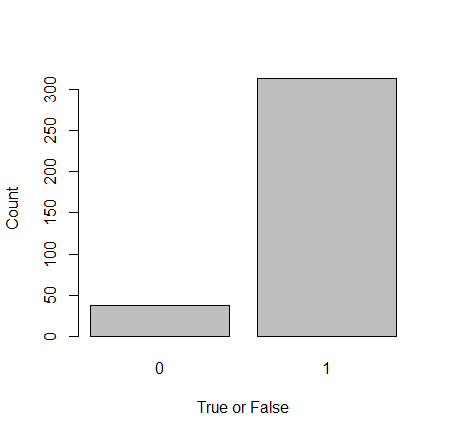
\includegraphics[width=100mm, scale = 0.5]{barplotV1.png}
  \caption{V1 barplot}
  \caption*{right skewed distribution}
\end{figure}
\begin{figure}
  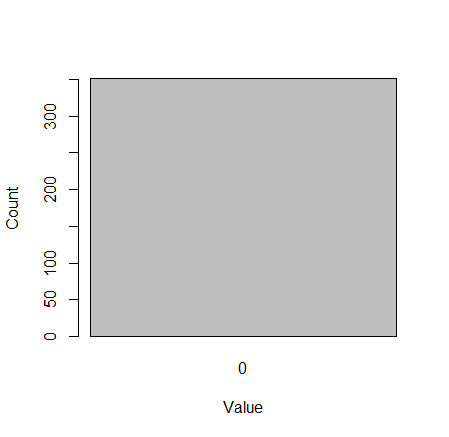
\includegraphics[width=100mm, scale = 0.5]{barplotV2.png}
  \caption{V2 barplot}
  \caption*{uniform distribution}
\end{figure}
\begin{figure}
  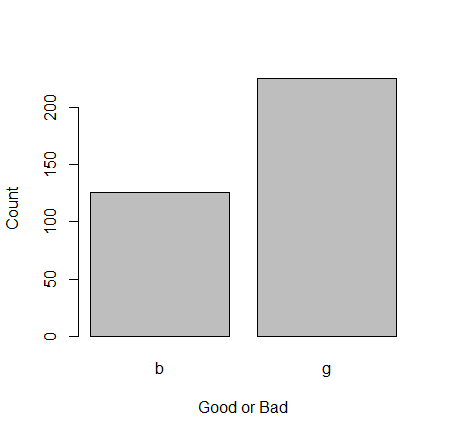
\includegraphics[width=100mm, scale = 0.5]{barplotV35.png}
  \caption{V35 barplot}
  \caption*{right skewed distribution}
\end{figure}
\begin{figure}
  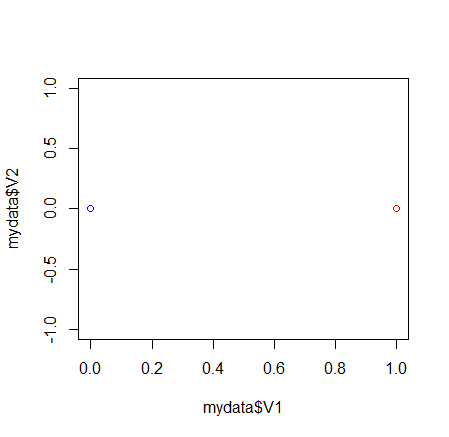
\includegraphics[width=100mm, scale = 0.5]{scatterplotV1V2.png}
  \caption{V1 V2 scatterplot}
  \caption*{There are only two points on the graph, "good" or "bad" value depends on variable 1, if V1 equals 1, then it is good value. If V1 equals 0, then it is bad value.}
\end{figure}
\begin{figure}
  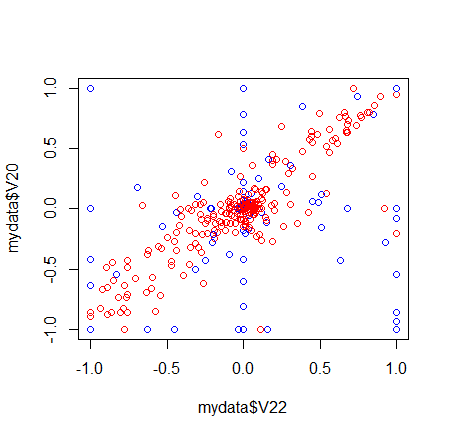
\includegraphics[width=100mm, scale = 0.5]{scatterplotV2022.png}
  \caption{V20 V22 scatterplot}
  \caption*{All the good value are linearly correlated, and the bad values are not correlated}
\end{figure}
\end{enumerate}
%%%%%%%%%%%%%%%%%%%% PROBLEM 2  %%%%%%%%%%%%%%%%%%%% %%%%%%%%

\section*{Problem 2 [10 points]} 

The pseudo-code for $k$-means and a running example of $k$-means on a small data set are provided above. Answer the following questions:

\begin{enumerate}
  \item[2.1] Does $k$-means always converge? Given your answer, a bound on the iterate must be included. How is
its value determined?
\paragraph{}
By definition, $k-means$ always converge. Given a data set, we first initialize $n^{th}$ random centroids and set a termination condition, then assign data point to its closet centroid. Check whether the data meets the termination condition (after $i^{th}$ iteration or already optimitized). If the condition is not met, find the mid point of each centroid data set, and repeat steps above.
  \item[2.2] What is the run-time of this algorithm?
\paragraph{}
Let n be the number of data point, i be the number of iteration. Complexity is O( n * K * I * d ), n = number of points, K = number of clusters, I = number of iterations, d = number of attributes
\end{enumerate}


%%%%%%%%%%%%%%%%%%%% PROBLEM 3  %%%%%%%%%%%%%%%%%%%% %%%%%%%%


\section*{Problem 3 [20 points]} 

 Implement Lloyd's algorithm for $k$-means (see algorithm $k$-means above)  in \textit{R} and call this program $C_k$. As you present your code explain your protocol for


\begin{enumerate}
  \item[3.1] initializing centroids
  \item[3.2] maintaining $k$ centroids
  \item[3.3]  deciding ties
  \item[3.4] stopping criteria
\end{enumerate}



%%%%%%%%%%%%%%%%%%%% PROBLEM 4 %%%%%%%%%%%%%%%%%%%% %%%%%%%%

 
\section*{Problem 4 [40 points]}
 
 In this question, you are asked to run  your program, $C_k$, against   \href{https://archive.ics.uci.edu/ml/datasets/ionosphere}{
Ionosphere Data Set}. Upon stopping, you will calculate the quality of the centroids and of the partition.  For each centroid $c_i$, form two counts:
  \begin{eqnarray*}
  g_i &\gets& \sum_{\delta \in c_i.B} [\delta.C =\text{\quotes{g}}],\ \ \ \mbox{\rm good}\\
  b_i &\gets& \sum_{\delta \in c_i.B} [\delta.C = =\text{\quotes{b}}], \ \ \ \mbox{\rm bad}
  \end{eqnarray*}
  where $[x = y]$ returns 1 if True, 0 otherwise.  For example, $[2 = 3] + [0 = 0] + [34 = 34] = 2$
  
  The centroid $c_i$ is classified as good if $g_i > b_i$ and bad otherwise.  We can now calculate a simple error rate.    Assume $c_i$ is good.  Then the error is:
 \begin{eqnarray*}
 error(c_i) &=& \frac{b_i}{b_i + g_i}
 \end{eqnarray*}
 We can find the total error rate easily:
 \begin{eqnarray*}
 Error(\{c_1, c_2, \ldots, c_k\}) &=& \sum_{i=1}^k error(c_i)
 \end{eqnarray*}
\begin{figure}
  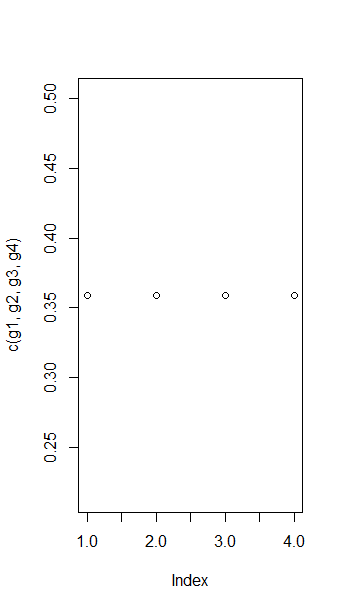
\includegraphics[width=100mm, scale = 0.5]{error.png}
  \caption{SSE}
\end{figure}
\paragraph{}
Report the total error rates for $k = 2,\ldots 5$ for 20 runs each, presenting the results that are easily understandable.  Plots are generally a good way to convey complex ideas quickly, i.e., box plot.  Discuss  your results.\\
As we can see from the graph, No matter how many clusters there are, the error rate will always be the same.\\


%%%%%%%%%%%%%%%%%%%% PROBLEM 5  %%%%%%%%%%%%%%%%%%%% %%%%%%%%

 
 \section*{Problem 5 [10 points]} In this question, you are asked to make use of  the \href{https://stat.ethz.ch/R-manual/R-devel/library/stats/html/kmeans.html}{ R package for $k$-means.} Elbow method is one of the techniques to decide the optimal cluster number.  Find the optimal cluster number for Ionosphere data set using elbow method (for  $2 \leq k \leq 15$). Provide a plot that shows the total SSE for each $k$. Discuss your results.
\begin{figure}
  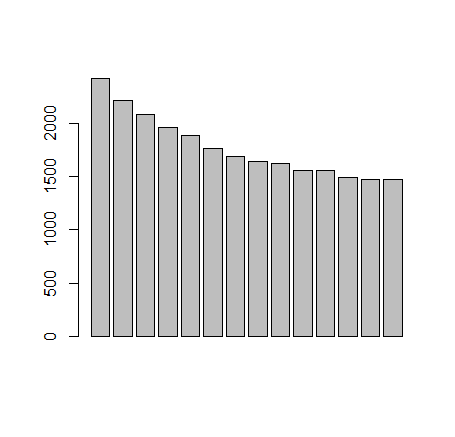
\includegraphics[width=100mm, scale = 0.5]{SSE.png}
  \caption{SSE}
\end{figure}
%%%%%%%%%%%%%%%%%%%% PROBLEM 6  %%%%%%%%%%%%%%%%%%%% %%%%%%%%
 
\section*{Problem 6 [10 points]}

Let $X \subset \mathbb{R}^n$  ($\mathbb{R}$ is the set of reals) for positive integer  $n>0$. Define a  distance $d: X \times X \rightarrow  \mathbb{R}_{\geq 0} $ as

\begin{equation*}
d(x,y) =  max\{|x_i - y_i|\}, \forall i\ 1\leq i \leq n
\end{equation*}

Prove/disprove $d$ is a metric?
\paragraph{}
$1. (Non negativity) : as |a-b| is always >= 0, it's True$\\
$2. (Definiteness): If |a-b| = 0, a must equals b. So this is True$\\
$3. (Symmetry): Since |a-b| = a - b = b - a. Therefore, d(x,y) = d(y,x)$\\
$4. d(x,y) \leq d(y,z) + d(x,z)$\\
$max{|x - z|} \leq max{|x-y| + |y - z|}$\\
$max{|x-y|} + max{|y-z|} = d(x,y) + d(y,z)$
%%%%%%%%%%%%%%%%%%%% Extra credit %%%%%%%%%%%%%%%%%%%% %%%%%%%%

\section*{Extra credit [30 points]}

This part is optional. 

\begin{enumerate}

\item[1] The $k$-means algorithm provided above stops when centroids become stable (Line  34). In theory, $k$-means converges once SSE is minimized
\begin{eqnarray*}
SSE = \sum_{j}^k \ \ \smashoperator{ \sum_{x \in c_j.B}} ||\mathbf{x} - c_j.v||^2_2 \label{costfunt}
\end{eqnarray*} 

In this question, you are asked to use SSE as stopping criterion. Run $k$-means over  \href{https://archive.ics.uci.edu/ml/datasets/breast+cancer+wisconsin+(original)}{ Breast Cancer Wisconsin Data Set} and report the total SSE  in a plot for $k = 2,\ldots ,5$ for 20 runs each. Discuss your results. [15 points].



\item[2] Traditional $k$-means initialization is based on choosing values from a uniform distribution. In this question, you are asked to improve $k$-means through initialization.  \href{http://ilpubs.stanford.edu:8090/778/1/2006-13.pdf}{$k$-means ++} is an extended $k$-means clustering algorithm and induces non-uniform  distributions over  the data  that serve as  the initial centroids. Read the paper and discuss the idea in a paragraph.  Implement this idea to improve your $k$-means program. [15 points]
\end{enumerate}

%%%%%%%%%%%%%%%%%%%%%%%%%%%%%%%%%%%%%%%%%%%%%%%%%%%%%%%%%%%%%%

\pagebreak
\section*{What to Turn-in}
 Submit a .zip file that includes the files below. Name the .zip  file as \quotes{usename-section number}, i.e., hakurban-B365.





\begin{itemize}
\item The *tex and *pdf of the written answers to this document.
\item *\texttt{R}files for:
\begin{itemize}
\item  implementation of $k$-means  [Problem 4] 
\item \texttt{R}  package  usage [Problem 5]
\item  extra  credit questions--optional
\end{itemize}
\item A README file that explains how to run your code and other files in the folder
\end{itemize}


 



\end{document}


